% General definitions; study-specific recipes are in experimental-study.tex.
% Operational provenance: methodology-notes.md. No empirical results.
\section{Methodology}
\label{sec:methodology}

\subsection{Sparsification interventions}
\label{sec:interventions}

A sparsification intervention specifies (i) where to set activations to zero
(thresholding sites $\mathcal{N}$), (ii) the thresholding function $G$, and
(iii) where to apply activation regularization pressure (pressure sites
$\mathcal{P}$). The sets $\mathcal{N}$ and $\mathcal{P}$ need not coincide,
and different sites may use different functions $G$. These choices give a
combinatorial set of interventions during training.

To avoid the overhead of exact top-$k$ selection~\citep{wang2024qsparse,you2025spark},
we extend ReLU to one-sided and symmetric thresholding:
$G_{+,\kappa}(x)=x\mathbf{1}\{x\geq\kappa\}$ and
$G_{\pm,\kappa}(x)=x\mathbf{1}\{|x|\geq\kappa\}$, with $\kappa\geq0$.
The threshold $\kappa$ controls thresholding strength and is fixed within each
training condition. Appendix~\ref{app:interventions} gives boundary and derivative conventions.

Figure~\ref{fig:pythia-block} locates the intervention sites: $a$ and $m$ are
the normalized inputs to the attention and FFN branches; $h$ is the FFN hidden
activation; $z$ is the concatenated attention context before output projection;
and $q,k,v$ are the query, key and value operands, with $q,k$ taken after RoPE.
The attention probabilities are denoted by $p$. We apply $G_{+,\kappa}$ at
selected sites among $a,m,h,z$ and $G_{\pm,\kappa}$ at $q,k,v$.
At $h$, the selected nonlinearity replaces GELU.

% Source artwork and observation: figures/pythia-architecture-map.tex and .md.
\begin{figure}[!htbp]
\centering
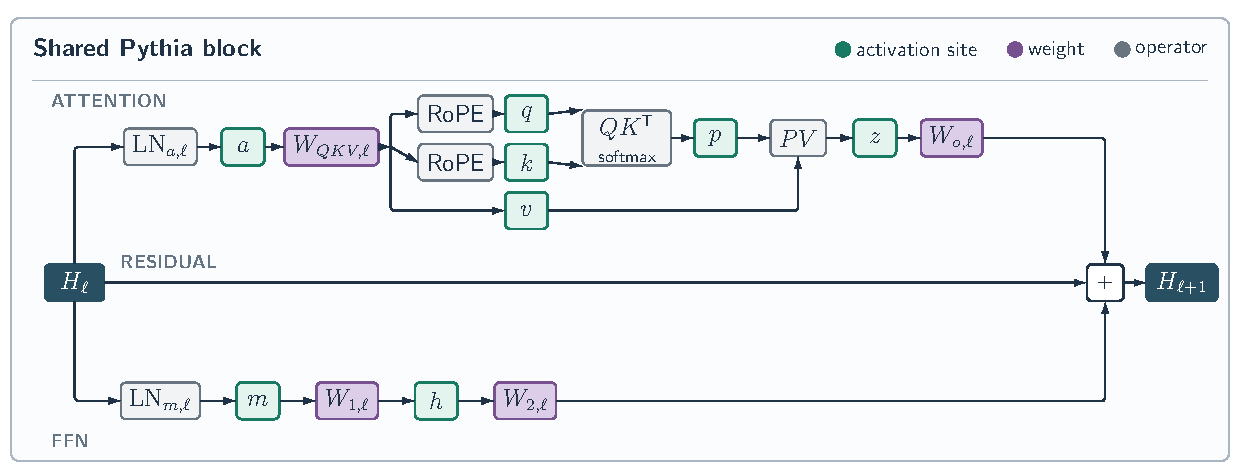
\includegraphics[width=\linewidth]{figures/pythia-architecture-map.pdf}
\caption{\textbf{Intervention sites in a shared Pythia block.}
Attention and FFN branches use separate LayerNorms and join the residual path.
Green nodes identify activation sites; purple nodes identify learned weights.
Table~\ref{tab:interventions} specifies thresholding and pressure assignments.}
\label{fig:pythia-block}
\end{figure}

For optimization pressure, $\mathcal{L}_1$ averages the mean absolute activation
equally across targeted site--layer tensors, after any thresholding.
\emph{Naive L1} (L1N) minimizes $\mathcal{L}_{\mathrm{task}}+\lambda\mathcal{L}_1$.
The weight $\lambda$ adds a tuning dimension that affects sparsity and quality,
as reported by ProSparse~\citep{song2024prosparse} and \citet{cetin2026sparser}.
To limit this sensitivity, \emph{orthogonal L1} (OL1) adapts gradient-conflict
projection~\citep{yu2020pcgrad,hsieh2024bloop} to the AdamW update.
After a task-only AdamW step, it preconditions the pressure gradient using the
task's second-moment estimates
and removes its conflicting component when it opposes the adaptive task direction.
A unit norm budget caps the pressure correction at that direction's norm,
before applying the learning rate. For a fixed optimizer state, the ideal
capped correction no longer grows with $\lambda$, motivating fixed-budget
comparisons across interventions. This bounds pressure without guaranteeing
preserved task loss; Appendix~\ref{app:pressure} defines the procedure.

\subsection{Sparsity and architectural reach}
\label{sec:measurement}

\emph{Activation sparsity} is the fraction of exactly zero entries at a named site.
To weight zeros by the work they affect, we define \emph{model-wide sparsity}
as $\Smodel=N_0/N_{\mathrm{model}}$, reported as $100\Smodel\%$. Here, $N_0$
counts scalar multiplications with at least one zero activation operand in
the declared transformer-block matrix products. $N_{\mathrm{model}}$ counts all valid multiplications
in those operations and the dense language-model head; the head receives no
zero credit. Counts are pooled before division. The percentage refers to this
declared multiplication workload, not all operations or elapsed time. We count
only causally valid pairs in a full, uncached sequence;
Appendix~\ref{app:accounting} gives the exact counters.

The \emph{model-wide sparsity ceiling},
$\Smax=N_{\mathrm{reach}}(\mathcal{N})/N_{\mathrm{model}}$, counts the fraction
of that workload whose zero operand is guaranteed by setting the selected
sites to 100\% activation sparsity, crediting each affected multiplication once. It depends on the architecture,
site set, and sequence length, but not pressure or a checkpoint. The ceiling
characterizes selected-site reach rather than sparsity achievable at acceptable
quality: observed $\Smodel$ also includes natural zeros outside that reach.
Appendix~\ref{app:ceiling} defines the reach accounting.
